%% This is an abbreviated template from http://www.sigplan.org/Resources/Author/.
\newcommand{\prash}[1]{{\color{blue} [Prasanth: #1]}}

\documentclass[acmsmall,review,authorversion]{acmart}
\acmDOI{}
%\acmJournal{PLACMP}
\acmVolume{CSCI 5535}
\acmNumber{Spring 2020}

\begin{document}

%%
%% The "title" command has an optional parameter,
%% allowing the author to define a "short title" to be used in page headers.
\title{The Name of the Title is Hope}

%%
%% The "author" command and its associated commands are used to define
%% the authors and their affiliations.
%% Of note is the shared affiliation of the first two authors, and the
%% "authornote" and "authornotemark" commands
%% used to denote shared contribution to the research.
\author{TBD}
\email{tbd@colorado.edu}
\author{TBD}
\email{tbd@colorado.edu}
\affiliation{%
  \institution{University of Colorado Boulder}
}


%%
%% The abstract is a short summary of the work to be presented in the
%% article.
\begin{abstract}

\textcolor{blue}{
\begin{enumerate}
  \item What is the technical problem you are addressing?\\
  We intend to explore one method of compositional testing of protocols used in the control-plane of cellular communication infrastructure. 
  \item Why is addressing the problem important? \\
The architecture and design of the cellular-communication-network is fast evolving to handle the needs of IoT and 5G communication. With the increase in scale, comes the need to update the different protocols used to control-coordinate decision making in the control-plane. While the protocols get updated, the implementations of the protocols need to be evaluated for compliance with older versions, for the sake of backward compatibility. Current methodoly of testing doesn't help to address this challenge. 
\item Why is solving this problem hard? \\
There has been an interest in the community to adopt formal methods to specify and to ensure correct implementations of protocols within the software and internet-network domain. There hasn't been any prior work that does this within the cellular domain. The current intention is not provide a formal-translation of the natural-lanaguage specification, but rather to provide an on-the-wire specification of the protocol, with little or no emphasis on the internal-mechanisms that are to be satisfied by the different entitites. 
\item What is your expecgted contribution?\\
Ourr contribution is to transfer the tools and techniques that's being adopted for internet-protocols, to the domain of control-plane protocols within cellular communications, with a particular focus on the interaface between the Radio part and the Core part of the network. 
\end{enumerate}
}

\textcolor{green}{
\begin{enumerate}
\item What is the problem? \\
We intend to provide a formal specification of the S1AP protocol that forms the basis of communication between the Evolved Packet Core (EPC) of the cellular communications core network and E-nodeB (base-station) and use this specification to generate automated randomized testers for implementations of S1AP.
\item Why is the problem important?\\ 
 If the implemented code does not exactly follow the protocol, communication using the protocol cannot be correctly performed. However, it is not easy to write the code for the protocol because the protocol definition document is complicated.
 \item Why is the problem hard? \\
 This is because we need to understand the complex protocol, implement the code according to the developed IVy language for verification, and consider various error cases.
\item What is your contribution?\\
 Our automatic testers can quickly find errors in the S1AP implementation process to minimize errors that can occur in the actual communication process.
\item What follows from your contribution? \\
By building a correct LTE network simulation environment with S1AP protocol, we can perform research to improve network performance, such as speed improvement.
\end{enumerate}
}

\end{abstract}

%%
%% This command processes the author and affiliation and title
%% information and builds the first part of the formatted document.
\maketitle

\section{Introduction}

\textcolor{red}{
Introduction
- Define the problem and state the contributions. That is, expand the sentences from the abstract into paragraphs covering primarily questions 1-4.}

\prash{
Questions to address in introduction: 
\begin{enumerate}
\item What is the Cellular Core System? Which part of the system are you handling? 
\item What is S1AP? What is NAS? 
\item How is S1AP/NAS specified? 
\item What is the current process for determining the correctness of the protocol? 
\item What are the current issues? 
\item What do we need? 
\item what do we offer? Why is this more challenging? 
\item what shall you be implementing and demonstrating? 
\item what did you learn from this process? 
\item what are the drawbacks/negatives of this procedure? 
\end{enumerate}
}

\prash{
The 5G cellular network deployment, with the promise of enabling an internet-of-things and high-bandwidth, low-latency-applications, is an endeavour that has been the target of industrial players in the last few years. The promises of the 5G newtork architecture arises primarily from the follpwing enhancements over the 4G LTE architecture: (1) improvements in the physical and application layer technologies enabling large number of devices with higher bandwidth provisions, (2) enhanced security features introduced into the protocol stack. The 5G standard proposes a complex architecture of subsystems that interact with each other at different layers of the communication stack, while using multiple sub-procotols between entitites. 

The cellular network infrastructure may be viewed as a  large-scale wireless with a wired backend that is designed to support mobile data and voice services. Communication and messaging between the entities may be surmised under two layers of its design-abstraction called control-plane and data-plane. The control plane protocols form a significant part of its design, as it provides complex signalling functions, which makes it quite different from the network protocols that enable the internet. They follow the layered protocol architecture and run at both the network infrastructure and the end device. The cellular network control-plane, consists of a number of critical procedures(e.q. Initial UE Registration, UE Mobility, UE deregistration, etc) which are leveraged by the primary cellular services like paging, voice-call, SMS, data and billing. Incorrect implementations of the protcols can have adverse consequences to these services. 

The subset of the cellular network architecture we intend to focus on, comprises of the BaseStations(BS) and the core-network(CN). The BS provides radio-access to user-devices(UE), while the  CN connects them to the public-telephony network or the internet. The 4G/5G LTE network provides packet-switching data-services only. It is constituted of the following three entities: (1) Mobility Management Entity (MME), (2)Home Subscriber Server (HSS) , and (3) Gateways. The MME manages user mobility, and is the primary port-of-entry of all signalling from the radio-network to the core-network. The HSS stores the user-subscription information and the Gateways route packet-switched data-packets between the internet and the BS. 

In this work, we examine the protocol-specific interactions between critical components over the control plane, with an intention of identifying problems/mis-compliance of entitites to the protocol specifications. To be precise,  we intend to address the following concrete research question: \\
\textit{Is it possible to formally verify the correctness of a subset of the critical procedures handled by the control plane interactions between the EPC and the MME(cellular core network)?}\\

There are two key challenges to this endeavour - (1) compared to the internet, cellular networks are still closed systems i.e. signalling exchanges between devices and base-stations, or between the base-stations and the core-network are not readily accessible during normal operations, (2) patterns of inter-protocol communication over the control-plane are more diverse and complex, in comparison to their counterparts over the internet. Protocol interactions are visible not just at the inter-layer interfaces, as seen over the internet, but also in cross-domain (e.g data and carrier grade voice services require signalling for circuit-switching and packet-switching in these networks), and cross-system scenarios ( due to heterogenous deployment strategies inter-system switching between 3G, 4G and 5G systems need to be facilitated).
\\
}

  \begin{enumerate}
  \item Define the problem you'll solve :\\
  We intend to extend the applicatiton of Compositional Verification of Internet-protocols to the domain of celluar communication networks, with a specific focus on the interface between the e-NodeB and the Core-Network. Instead of translating the 3GPP protocol specification for the S1-Application Protocol(S1AP) and the Non-Stratum Access(NAS) protocol, we intend to demonstrate the methodology for specifying on-the-wire messages that are exchanged between the entities while interacting over a stateful-protocol. We shall focus on implementing one of the primary procedures facilitated by the EPC, the UE-Attach Procedure. In this procedure, the EPC facilities the connection of a UE(mobile phone/IoT device ) to the cellular network, to permit data-transmission over IP. 
  \item What is the general approach you intend to use to solve the problem? \\
  We intend to use the IvY tool for providing a formal-specification of the S1AP/NAS protocol. In addition, we intend to test the MME component(server) of the Core-Network while generating test-messages that shall be sent by the e-NodeB(Client, Radio-link). 
  \item Why do you think the approach will sovle the problem? \\
  This approach has been successfully used to verify a complex stateful internet-protocol, QUIC, which runs as an application-layer protocol, while using UDP to send/transmit messages over the network. This use case is very similar to the domain of cellular-communication networks, where the control-plane protocols are executed as application-layer protocols, executing over an underlying SCTP transport-layerr protocol, which is used to communicate messages on-the-wire. 
  \item How do you plan to demonstrate the idea? \\
  We plan to demonstrate it by encoding the specification of the protocol in the IvY tool, and to adopt its automated-test-message generation process to evaluate some open-source implementations of cellular-core-network ( e.g OpenEPC ). 
  \item How will you  evaluate your idea? What will be the measure of success? \\
  The measure of success would be the following: 
  \begin{enumerate}
  \item Implementation of SCTP transport protocol within IvY, to facilitate message transmisison between the IvY system and the EPC-implementation(server). The functionality shall be evaluated by the ability to transmit "S1-Setup Request Message" and also to receive "S1-Setup Response" message.
  \item Specification of subset of S1AP/NAS protocol that enables the "UE-Attach Procedure". This shall be evaluated by a successful simulation of a UE-Attach by an arbitrary UE with the EPC. 
  \end{enumerate}
  \end{enumerate}


\section{Overview}
\textcolor{red}{
Overview
- Showing your contribution through an example (and a bit of why hard).
}

\subsection{LTE Preliminaries}

In the following subsection we shall cover some aspects of the cellular network system, with an emphasis on the sub-systems that we shall be targetting our testing procedure on. 

\subsubsection{LTE Network Architecture}
As mentioned earlier, the LTE network architecture is broadly constituted of three components: (1) the cellular device, (2) the radio access network(BS, and radio channels), (3) the evolved packet core or the core-network(CN and the wired communication channels between the BS and the core). 

\textbf{User Equipment(UE)}: The end-user communication device which is equipped with a Universal Subscriber Identity Module known as the SIM card, serves as a terminal device(UE). The SIM contains unique identification information for each subscriber, of which the following two parmeters are vital: (1) the international mobile subscirber identity (IMSI) number, and (2) the international mobile equipment identity(IMEI) number, apart from the associated cryptographic keys that are required to ensure security and privacy protection of various interaction-procedures with the network. 

\textbf{Base Station(BS)}: The cellular network radio-acess network, partitions the geographical space into hexagonal cells, to cater to the needs of subscribers within the region. Each geograhical cell is serviced by a single base-station, located at its 'center' , that acts as an intermediary connecting the geographically dispersed subscribers with the core-network. The E-UTRAN refers to the network between an eNodeBs(Base-stations) and the UEs. 

\textbf{Core-Network(CN)}: The core-network(CN) or the evolved-packet core(EPC) consists of the following primary entities: \\
(1) Mobility Management Entity: The MME serves as the primary interface between the radio-access network and the core-network. It manages the primary procedures of UE attach, UE detach, paging, etc, apart from the vital role of handling the mobility requriements of the UE. 
(2) Home Subscriber Server(HSS): The HSS component of a service-provider maintains UE identities and subscription details, apart from the cryptographic keys and information required for authentication of the entities. 
(3) Gateways: Once the control-signalling has established the authenticity of the UE, verified their subscription and established connection with the core-network, the Gateways handle the communication of data between the UE and the internet. 

\subsubsection{Initial UE Attach Procedure}
Of the set of vital control-procedures handled by the MME, we shall be focusing on the functionality and implementation of the Initial UE Attach Procedure. 

When a UE wants to connect to the EPC, which is automatically initiated by the device often when the device has been rebooted, it scans the radio-waves, to determine the eNodeB(base-station) with the strongest signal-power and attempts to establish a connection with it. The Initial UE Attach procedure, establishes a connection with the Base-Station, and triggers and subsequent connection to the core-network, by following the following four sequence of operations: 
\begin{enumerate}
\item Identification: The UE sends an Attach Request Message to the MME via the BS, by providing self-identifying information of its IMSI/IMEI and security capabilities. 
\item Authentication: On reception of the Attach Request by the MME, it forwards it to the HSS, to obtain an authentication of the UE, and also, generates an authentication challenge for the UE via an Authentication Request Message, so that it may authenticate the legitimacy of the MME it has established connection with. The UE uses its master cryptographic key to authenticate the MME and then on success, responds with an Authentication Response Message to the MME. If the authentication step is successful, the entities progress into the next stage of negotiating the security algorithm, to establish a secure channel of connection between them. 
\item Security Algorithm Negotiation: From the security capabilities avaiable in the UE, as communicated via the Attach Request message, the MME selects a security algorithm pairs(encryption and integrity), and communicates its choice to the UE along with the Message Authentication Code(MAC). Once the UE verifies the MAC, the UE and the MME establish a shared security context for protecting the secrecy and integrity of the messages transmitted over the channel in future. 
\item Secure Temporary Identifier Exchange: The MME then sends an encrypted and integrity-protected Attach Accept Message, which includes a temporary identity called GUTI(Globally Unique Temporary Identity) which shall be used as an identifier-pseudonym for the UE. This is introduced to reduce the exposure of sensitive information like the IMSI/IMEI to potential evesdropping and security-vulnerabilities in the system. The UE concludes the Attach Procedure, by transmitting an Atttach Complete Message to the MME followed, by the establishment of a  security context between the BS and the UE. 
\end{enumerate}

\subsection{Specification Methodology }
In this section, we present the specification methodology using examples. To specify the S1AP control-plane messaging protocol between the Base-Station(BS) and the MME, we shall use an abstract machine that monitors the protcol events. Conceptually, this machine observes the sequences of message interactions between the two communicating entities( tester and target) by observing the protocol-events triggered by the messages on the wire at the interface between the tester and the network. 
\textcolor{red}{The network is not explicitly modelled in this approach, though there's an assumption that the network may delay or drop or re-order messages, but it shall not create new messages. }
When an event occurs, the abstract machine (which isn't finite state by design) consults its state-representation to determine whether the event conforms to the protocol specification. If so, it updates its state to account for the event, else, \textcolor{red}{it may either marks the occurrence of an illegal event, or ignore it.} 

The protocol specification and the monitor are encoded in a language called Ivy. In Ivy, the events associated with messge-packets are modelled by an \textit{action}. Constraints may be imposed upon the state and the parameters upon an event, by defining  some conditions to be satisfied as a pre-condition or a post-condition. If these constraints are satisfied, the event is legal according to the protocol. Else, the events may be considered to be in violation of the protocol. 

The protocol state is represented by a collection of functions or relations. The choice between the functional-representation or the relatonial-representation is based on how the state-information shall be queried in downstream actions. The two forms of representation are conceptually equivalent. Any element of the relational-set represents a predicate-abstraction of the actual event. 

The properties of the protocol can thus be verified by the communication of abstracted messages between the entities, or it may be used to generate actual messages on the wire, using a \textit{shim} that generates actual network-protocol encoded messages to be sent on the wire, while also capturing the packet events received by the entitiy by tracing packets on the wire. While doing so, the shim triggers the specific protocol-events that get recorded as state-updates within the monitor. It is important to note that the specification is an executable monitor that observes the behaviour of all protocol nodes, in contrast to being an abstract implementation of the protocol entities. 

An important capability provided by the Ivy tool, is the capacity to obtain a \textit{generator} that produces random sequences of events that conform to the specification. The generator uses an SMT solver to randomly select a valuation of parameters that satisfy the 'require' constraints enconded in the pre-condition of the selected action. Consequently, the generator helps to generate a random sequence of packet-events in compliance with the protocol-specification that is sent to the test-target. 

The S1AP application protocol messages are communicated between the eNodeB and the MME, based on a lower-layer transport protocol based in SCTP( in comparison to UDP or TCP for general data packets over the internet ). We create a shim that connects the abstract packet events to actual SCTP packets on the wire. The \textit{send} and \textit{receive} events are encoded within the shim. The shim is thus an ad-hoc mechanism that connects abstract protocol events of the specification to real-events in the system. Thus, if the socket or other implementation details of the system gets modified, the shim alone may be modified, without altering the protocol specification. This shim, thus helps us to connect the abstract protocol specification, to the physical resources such as the operating system, the networks and compilers to test real-world implementations. \textcolor{red}{It may also be modified to conduct experiments in a simulated environment based on NS3, or be used alone to conduct a formal analysis of the protocol in an abstract theoretically-sound manner. }

The specification may be encoded at a global level, accounting for all the roles that different protocol-entities may play, or at a role-based level, where only the specifications for a single-role are encoded. In the latter case, one needs to effectively assume that the role-being-modelled generates events that are correct according to the protocol, since it's the task of the generator to create the corresponding messages. The task of the verification process is to "guarantee" the correctness of events generated by counterparts of the tester i.e roles played by the be multiple(or single) test targets as required by the protocol design. This framework of Assume/Guarantee specification based testing has an inpmortant formal property: if the composition of roles ever violates the specification, then tehre must exist a failing assume/guarantee test for one of the many roles within the protocol. 

\subsection{Specification Examples}
This section shall be updated after we've had some progress in using the tool to model the messsages. 

\section{(Contribution 1)}

\section{(Contribution 2)}

\section{Empirical Evaluation}

\section{Properties previously tested in 4G/5G LTE Protocol Verification}
The following are extracts from the papers that describe the methodology with an emphasis on the properties they have considered. 
\subsection{LTEInspector}
This work proposes a systematic model-based adversarial testing approach that leverages the use of a symbolic model-checker and and a cryptographic protocol verifier for analyzing 3 critical procedures of the 4G LTE network. 

LTEInspectorconsiders the standard symbolicadversary model (alternatively known as the Dolev-Yao model ) for its analysis.

 LTEInspector takes the relevant 4G LTEabstract model  and a desired property , and tries to find a violation of $\phi$ in the model. The set of properties that LTEInspectoraims to check include authenticity(e.g., disallowing impersonation), availability(e.g., preventing service denial), integrity(e.g., restricting unauthorized billing), and secrecy of user’s sensitive information (e.g., preventing activity profiling).
 
 As a prerequisite of LTEInspector’s analysis, we first construct the 4G LTE ecosystem model by consulting thestandard specification document.  Our model captures the abstract functionality (ignoring low-level implementation details)of the 4G LTE ecosystem as synchronous communicating finite statemachines (FSM). Each FSM captures the stateful functionalityof a protocol participant’s (i.e, user’s cellular device and thecore network) at the Non-Access Stratum (NAS) protocol layer. The two FSMs communicate with each other through public (adversary-controlled) communication channels by sending each other NAS layer messages.
 
Checking complianceof the protocol model against desired security and privacyproperties often requires simultaneously reasoning about:
\begin{enumerate}
 \item temporal ordering of different events/actions (i.e., trace properties such as response properties [21]), 
\item cryptographically-protected messages and constructs (e.g., encryption, hashing),and 
\item  other rich constraints (e.g., linear integer arithmeticconstraints).
\end{enumerate}
LTEInspector lazily (or, on an on-demand basis) combines the reasoning powers of a symbolic model-checker and a cryptographic protocol verifier. 

\textit{Use of Model-checker}
 In this approach,we first abstract away all cryptography-related constructs from the model M and the desired property $\phi$. For any violation of the reduced property,  the symbolic model checker would yield a counterexample $\pi$ demonstrating the violation. 

\textit{Use of Cryptographic Protocol Verifier}
The counter-example $\pi$ may include adversary actions which may not be realizable due to cryptographic assumption violations (e.g., constructing avalid ciphertext of a message without possessing the encryptionkey). To rule out such cases, for each adversary action in $\pi$, we query a cryptographic protocol verifier to check the action’s feasibility with accordance to the cryptographic assumptions.In case all adversary actions in $\pi$ turn out to be feasible, we can report $pi$ to be a feasible vulnerability. If, however, there exists one adversary action in $\pi$ which is not feasible, we refine theproperty $\phi$abs to rule out traces in which the adversary takes that action. The analysis is then run again with the refined property. For further confidence, we validate $\pi$ by concretely executing it in a testbed.

\textit{Properties}
We have tested the Model against 14 properties in total in which 7 properties were analyzed with NuSMV(symbolic model-checker) whereas 7 properties were analyzed with ProVerif( cryptographic protocol verifier).

\begin{enumerate}
\item $\phi_1$: It is always the case that whenver the UE FSM is in the wait for the auth-request state, it will eventually move to the state where the UE authenticates the MME. 
\item $\phi_2:$( refinement over $\phi_1$) Once UE FSM moves into the wait-state for the auth-request, the environment will never set the value of the mobile-restart to be true. 
\item $\phi_3:$(refinement over $\phi_2$) mac-failure is never set to true by the environment
\item $\phi_4:$(refinement over $\phi_3$) UE FSM never receives the detach-request message. 
\item $\phi_5 :$(refinement over $\phi_4$) UE FSM never receives the auth-reject message
\item $\psi_1 :$( CPV Property) Every attach-request message received by the MME should be preceded by a unique attach-request message sent by the UE. 
\end{enumerate}

\begin{figure}[H]
    \begin{center}
        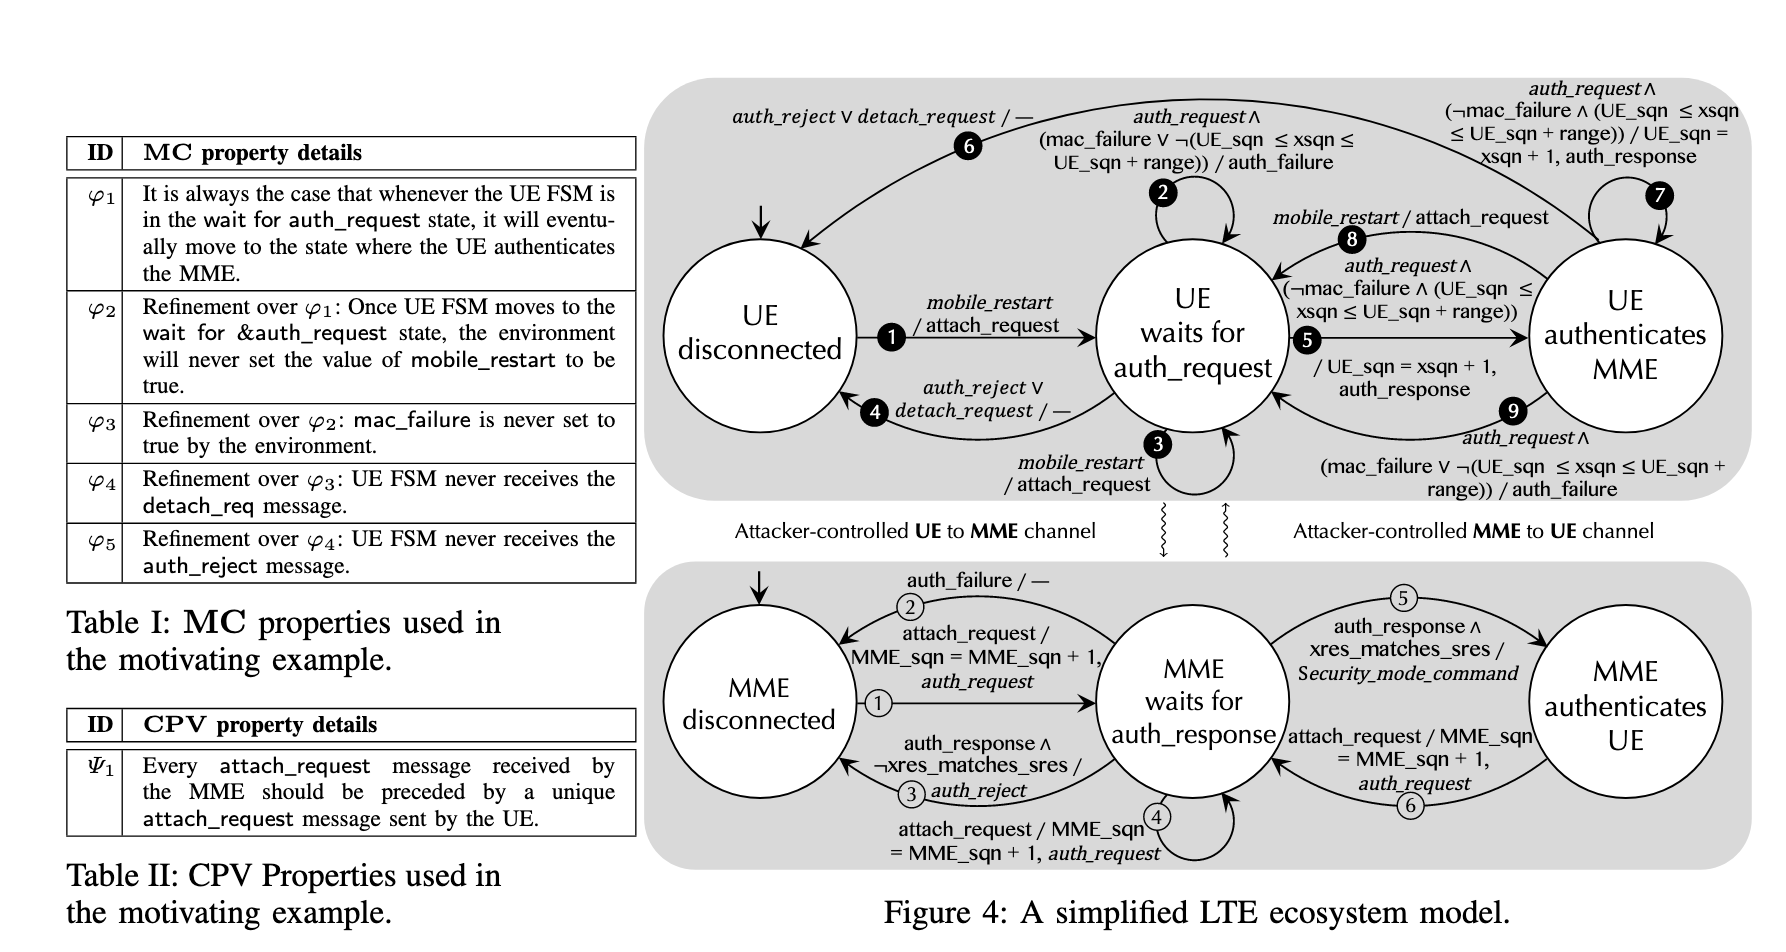
\includegraphics[width=0.7 \columnwidth]{./images/LTEInspector} 
    \end{center}
    \caption{Initial UE Attach procedure (will be changed)}
    \label{fig:inital-ue-attach}
\end{figure}

\paragraph{Criticism: The authors do not handle a comprehensive verification of the system, but rather introduce a procedure that may be followed for formal verification of the protocols. They then substantiate their formal methodology, by introducing and explaining different attack-vectors for the sake of discussing the ways in which the formal-verification methodology guided them in creating the vectors. 
}

\subsection{5GReasoner}
In this tool, the authors adopt a procedure similar to LTE verify, but use different tools, and formulate different properties, which are similar to the one's handled/addressed in the earliier work. So, apart from the numeric count of the properties that are verified, its critical to examine which properties are fundamentally important for the system. 

The enumerate the total number of properties that have been verified, but they do not provide a description of the language in which the properties have been specified. 
The end the work, by describing the different network-attacks that they claim, have been identified through the process of the formal-verification procedure. 

Sources for specification propeties:
\begin{enumerate}
\item conformance test-suites : NAS Layer: total 74 ( 9: liveness, 65: safety); RRC Layer: total 63( 6:liveness, 57: safety )
\item technical-requirement document 
\item technical-specification document:  total 50 properties ( 33: liveness; 17: safety) 
\end{enumerate}

Since the models are represented using FSM, it has to be the case that the properties have been modelled using Temporal Logic. 

To test a UE’s correct behavior in dif-
ferent control-plane procedures, the 3GPP standard defines confor-
mance test cases from the UE’s point of view. (5G; User Equipment (UE) conformance specification; Part 1: Protocol (3GPP
TS 38.523-1 version 15.3.0 Release 15)) 

We break down the high-level test case into fine-grained sub test-cases by enumerating all possible conditions, and then translating them into formal properties.

\textit{Capturing Data and Packet Payload}\\
One of the main challgens in formal verification of the protocols is the capture and generation of packet-payloads. 

Modelling predicates over the data
\begin{enumerate}
\item Validity Predicate: validity of authentication codes, not the exact value. 
\item Presence predicate: one-hot encoding
\item Grouping predicate: 
\item Timer predicates: Booleans for start and timeout 
\end{enumerate}


\section{Related Work}

\prash{
We attempt to extend the formal specification based testing methodology introduced in \cite{} to the domain of control-plane application layer protocols. In \cite{}, while describing the experience of verifying the QUIC protocol, the authors have reviewed the different approahces to generating adversarial tests for network protocols. Some of the methods can be summarized as follows. 

We may observe a taxonomy of classification of the approaches for testing network-protocols as constituting of two main branches, one based on formal specifications and the other not based on formal specification. 
The latter branch consists of methods like "fuzz testing", in which , and "white-box testing", in which one extracts traces of the internal control flow paths of the target system,that is then used to discover input-values(via SMT solvers or symbolic execution methods) that stimulate code-branches that were previously ignored.

One of the testing frameworks based on formal specification of the protocols, include model-based testing(MBT) and its precedents within the field of protocol-conformance testing. The protocols are specified as finite-state machines(FSMs), which are then explored to generate test-scenarios in an online or offline operational scenario. These methods require procedures to fill in concrete data parameters of messages, which leads to significant complexity in these formalisms. 

The compositional testing methodology, introduced in \cite{}, does not model the protocol as a FSM. It instead, adopts a constrained-random approach to generating tests based on an assume-guarantee formulation, which is a non finite-state specification. Further, the approach focuses on developing a global representation of the protocol, rather than separate specifications based on the role of an entity within the protocol. In this way, a single specification is used for the generation of tests to verify targets playing different roles within the protocol. By adopting an assume-guarantee based specification for the protocol, as used within the domain of program-analysis, this methodology avoids the constraint of general finite-state machine models to describe only some restricted aspect of the protocol. Though, the assume-guarantee/compositional testing methodology has been used successfully for software and hardware verification, it's application to the network-protocol verification faces new challenges introduced by the presence of data which constitutes the specification state and the messages. 


An alternative to using a testing-methodology for examining the correctness of a network protocol, is to construct formally verified reference implementations or to prove properties of an existing implementtaiton. These implementations are assumed to be built to compliance to a reference standard specification. They only way they can be used to guarantee compliance to a common standard, is when they are used as targets within an interoperability testing framework. 

Another alternative to examining the correctness of protocols, is to infer protocol specifications from message traces that are recorded on the wire. In the Network Semantics Project, the formal specification is used as a test-oracle to examine the compliance of observed message traces. In a similar vein, there has been prior work in which software API specifications, restricted to a finite-state abstraction, have been inferred automatically from run-time traces. 

The above alternatives to proving correctness of network protocols, stands apart from the larger body of work related to the abstract modeling and analysis of network protocols, in that they are more grounded to practice and examining real-world systems. The latter theoretical approaches are often confined to asserting theoretical properties of the system, which is often separated from any concerns of a workable system in practice. 

}

\prash{ Work related to verification of cellular network protocols\\

CNetVerifier \cite{} is a tool to analyse the inter-layer, inter-domain and inter-system protocol interactions within the control-plane of cellular communciation networks. The tool adopts a model-checking methodolgy within its two-phase protocol-diagnosis strategy to detect issues arising from (1) design problems within the protocol standards specification, and (2) operational mistakes of the service-provider. The verification strategy, however, is user-centric, i.e. the properties that are verified is related to the user-entities and cannot be used to examine interactions between the BS and CN, which would be of interest to improve the operational needs of the carrier/service-provider.  In this work, the protocol is modelled as two interacting FSMs, with one representing the UE, and the other representing the network entity( BS, MME, etc), within the model-checking framework, SPIN. The measurement based verification is handled at the UE level. 
\\
\\
LTEInspector \cite{} which employs a property-driven adversarial model-based testing philosophy. LTEInspectortakes the relevant 4G LTE abstract model and a desired property ($\phi$), and tries to find aviolation of $\phi$ in the model. The tool checks for the following properties  - authenticity, availability, integrity, and secrecy , all from the perspective of the end-user/customer. The model they develop comprises of as synchronous communicating finite state machines which abstract away the functionality while ignoring low-level implementation details. 
They adopt an instance of the parameterized system verification problem (i.e., parameterized by the number of protocol participants).Their instantiation of the LTEInspector framework, however,adopts the following constraints: (1) They consider only a
single layer of the protocol stack in isolation; (2) For
the sake of scalability, they only model packet type and do not
model critical data or packet payload, missing out on interesting
data-/payload-dependent protocol behavior; (3) Their adversary
instantiation cannot handle protocols spanning across different
layers of the stack. \\ \\
In the most recent work, 5GReasoner, the authors adopt a modelling procedure which models about five different control-plane procedures, with a FSM modelling each layer of the stack. The state-machines corresponding to different entities communicte via a public, adversary-controlled channel, where the adversary is also modelled as a FSM. The NAS layer protocol packets which constitute data-packets of the RRC layer protocols, is modelled using a behaviour-specific predicate-abstraction methodology, in which they do not directly model the data, but only predicates-over the data which are essential to verify the specific properties they are examining. These models are implemented in two infinite-state model-checkers and a cryptographic protocol verifier. They have verified about 187 properties which were extracted either from the standards, or were specified based on domain-knowledge

}

\prash{Questions/TODO: 
\begin{enumerate}
\item What are the works related to Testing of Cellular Application Protocols?
\item What does it mean to check for compliance with a common standard? How is that guaranteed by the compositional testing methodology? 
\end{enumerate}
}


\prash{ To be reviewed: \\
  The primary research exercise that we undertake is to determine an good methodology for providing a formal-specification for the control-plane protocols used in the cellular communication infrastrucuture. When we think about task for formalizing a specification for a protocol, there are two main use-cases: (1) to use the specification as an input for verifying that a particular model of its implementation satisfies some desriable properties, and (2) to enable the development of correct by construction implementations of the protocol. In our work, we explore the domain of specification as a means to conduct testing of an implementation, by facilitating a mechanism of automated generation of test-messages that shall be used to test the communication interface between two entities. Most of the related research have focused on the issue of formal-verification of correctness and security properties that are provided by the authentication protocols used in this domain. A formal methodology of testing of a communication protocol has been attempted within this domain. An interesting research project, that aligns with our endeavour, is the Project Everest, which attempts to create a formally verified stack to guarantee verified low-level implementations of the HTTPS stack. }
  
\section{Conclusion}

%%
%% The acknowledgments section is defined using the "acks" environment
%% (and NOT an unnumbered section). This ensures the proper
%% identification of the section in the article metadata, and the
%% consistent spelling of the heading.
\begin{acks}
TBD
\end{acks}

%%
%% The next two lines define the bibliography style to be used, and
%% the bibliography file.
\bibliographystyle{ACM-Reference-Format}
\bibliography{paper}
\end{document}
